\documentclass[12pt, a4paper]{article}

\usepackage[utf8]{inputenc}
\usepackage[T5, T1]{fontenc}
\usepackage[english]{babel}
\usepackage{geometry}
\usepackage{graphicx}
\usepackage{xcolor}
\usepackage{amsmath, amsfonts, amsthm}
\usepackage{listings}
\usepackage{hyperref}
\usepackage{parskip}
\usepackage[normalem]{ulem}
\usepackage{url}
\usepackage{fancyhdr}
\usepackage{lastpage}
\usepackage{titlesec}
\usepackage{enumitem}
\usepackage{tikz}
\usetikzlibrary{positioning, shapes.multipart, arrows.meta}
\usepackage{float}

\geometry{a4paper, margin=0.75in, top=1in, bottom=1in}

\definecolor{dkgreen}{rgb}{0,0.6,0}
\definecolor{dred}{rgb}{0.545,0,0}
\definecolor{dblue}{rgb}{0,0,0.545}
\definecolor{lgrey}{rgb}{0.9,0.9,0.9}
\definecolor{gray}{rgb}{0.4,0.4,0.4}
\definecolor{darkblue}{rgb}{0.0,0.0,0.6}

\lstdefinestyle{mystyle}{
    language=C++,
    basicstyle=\ttfamily\small,
    keywordstyle=\color{blue},
    commentstyle=\color{green!60!black},
    stringstyle=\color{red},
    numbers=left,
    numberstyle=\tiny,
    breaklines=true,
    frame=single,
}
\lstset{style=mystyle}

\lstdefinelanguage{cpp}{
  backgroundcolor=\color{lgrey},  
  basicstyle=\footnotesize\ttfamily\color{black}\bfseries,   
  breakatwhitespace=false,       
  breaklines=true,               
  captionpos=b,                   
  commentstyle=\color{dkgreen},   
  deletekeywords={...},          
  escapeinside={\%*}{*)},                  
  frame=single,                  
  language=C++,                
  keywordstyle=\color{purple},  
  morekeywords={BRIEFDescriptorConfig,string,TiXmlNode,DetectorDescriptorConfigContainer,istringstream,cerr,exit}, 
  identifierstyle=\color{black},
  stringstyle=\color{blue},      
  numbers=right,                  
  numbersep=5pt,                  
  numberstyle=\tiny\color{black}, 
  rulecolor=\color{black},        
  showspaces=false,               
  showstringspaces=false,        
  showtabs=false,                
  stepnumber=1,                   
  tabsize=5,                      
  title=\lstname,                 
}

\hypersetup{
    colorlinks=true,
    linkcolor=blue,
    filecolor=magenta,      
    urlcolor=blue,
    pdftitle={Project: Super Mario - Finals},
}

\pagestyle{fancy}
\fancyhf{}
\renewcommand{\headrulewidth}{0.6pt}
\renewcommand{\footrulewidth}{0.6pt}
\setlength{\headheight}{28pt}
\fancyhead[C]{HCMUS, VNU-HCM | 25A01, CS202: Finals, \textit{SuperMario} \\ Group 05}
\fancyfoot[C]{Page \thepage\ of \pageref{LastPage}}

\title{Project: Super Mario \\ 
\textit{Finals}}

\author{Khang N.D., Huy N.D., Nhat L.M., Thanh B.V., Thuy V.M.}

\date{2$^{nd}$ of September, 2026}

\begin{document}

\maketitle

\noindent \newline
\noindent \newline
\noindent \newline \makebox[\textwidth]{
\includegraphics[scale=0.3]{images/logohcmus.png}}

\newpage

\section*{Abstract}
Object-Oriented Programming (OOP) is a foundational paradigm in Computer Science for building robust, modular software systems. Developing a 2D platformer like \textit{Super Mario Bros.} provides an ideal framework for applying key OOP principles - such as inheritance, encapsulation, polymorphism, and abstraction - alongside foundational software design patterns. This project introduces a 2D game engine built in C++ using the SFML library, featuring a deterministic fixed-timestep game loop, stack-based state management, dynamic custom map parsing, and responsive character physics.

\subsection*{Purpose}
This project provides a modular, extensible 2D platformer clone of \textit{Super Mario Bros.} built in C++ using SFML, designed to demonstrate core Object-Oriented Programming principles and software design patterns in game architecture.

\subsection*{Key features}
The platformer incorporates a comprehensive suite of systems and gameplay mechanics:
\begin{itemize}
\item \textbf{Player Mechanics \& Characters}: Supports multiple selectable characters - Mario and Luigi - with custom movement, jumping physics, and state transformations including Small, Super, Fire, and Star states.
\item \textbf{Diverse Enemy AI}: Features distinct enemy behaviors for Goombas, Koopa Troopas, Koopa Paratroopas, Hammer Bros, Lakitus, Spinies, and Bowser.
\item \textbf{Custom Map Parser}: Loads multi-area levels from custom text-based \texttt{.map} files supporting solid terrain, interactive blocks, warp pipes, moving platforms, and decorations.
\item \textbf{Engine \& Game State System}: Built on a fixed-timestep game loop and a stack-based state manager transitioning seamlessly between Menu, Play, and Game Over states.
\item \textbf{Design Pattern Integration}: Implements core software design patterns including State, Singleton, and Factory to achieve high modularity and maintainability.
\end{itemize}

\subsection*{Mission}
This project aims to demonstrate how clean Object-Oriented design, structured engine architecture, and software design patterns can be applied to solve complex interactive problems in 2D game development.

\subsection*{Contact}

DANG-KHANG NGUYEN: 25125017, \texttt{ndkhang2535@apcs.fitus.edu.vn}

DUC-HUY NGUYEN: 25125014, \texttt{ndhuy2526@apcs.fitus.edu.vn} 

MINH-NHAT LE: 25125032, \texttt{mnhatle2007@gmail.com} 

VIET-THANH BUI: 25125065, \texttt{bvthanh2542@apcs.fitus.edu.vn} 

MAI-THUY VU: 23125046, \texttt{vmthuy23@apcs.fitus.edu.vn}

\newpage

\tableofcontents

\newpage

\section{Introduction}

This report documents the design, architecture, and technical implementation of a 2D \textit{Super Mario Bros.} platformer game developed in C++ using the SFML multimedia library. Developed as a final project for the Object-Oriented Programming (OOP) course, the project demonstrates the practical application of core OOP principles - inheritance, encapsulation, polymorphism, and abstraction - alongside software design patterns including State, Singleton, Factory, etc.

\subsection*{Overview of the Report}
The purpose of this document is to serve as both a technical architectural reference for software engineers and a practical operational guide for players and level authors. The report covers the software stack from high-level engine management down to specific collision-handling mechanisms and enemy AI routines.

\subsection*{Report Structure \& Roadmap}
To help readers navigate through specific topics, this document is organized into the following sections:

\begin{itemize}
\item \textbf{Chapter 1  -  Introduction}: Contains the abstract, purpose, key features, mission statement, and structural guide for this report.
\item \textbf{Chapter 2  -  Project Architecture}: Outlines the Model-View-Controller (MVC) division, structural class diagrams, engine scaffolding (\texttt{AppEngine}, \texttt{StateManager}), global tracking (\texttt{GameManager}), and entity hierarchies.
\item \textbf{Chapter 3  -  Implementation Details}: Explains the technical execution of key mechanics, including the fixed-timestep loop, custom \texttt{.map} file parsing, tile/entity collision resolution, state transformations, and enemy AI routines.
\item \textbf{Chapter 4  -  Development Cycle}: Describes the development workflow, milestone phases, and technical notes accumulated during development.
\item \textbf{Chapter 5  -  Tools Used}: Outlines the development environments, CMake build pipeline, SFML framework, version control, and media asset sources.
\item \textbf{Chapter 6  -  Features}: Details mandatory gameplay capabilities (3-level progress, sound effects, AI) and advanced features (such as character selection between Mario and Luigi).
\item \textbf{Chapter 7  -  Installation}: Provides instructions for setting up dependencies, configuring CMake, compiling the source code, and launching the executable.
\item \textbf{Chapter 8  -  Usage}: Serves as a manual covering player controls, power-up state transitions, warp pipe navigation, and the symbol reference for authoring custom map files.
\item \textbf{Chapter 9  -  Conclusion}: Summarizes project outcomes, known technical limitations, and prospective future enhancements.
\item \textbf{Chapter 10  -  References}: Lists core academic textbooks, API documentation, and technical reference wikis used.
\end{itemize}

\subsection*{Finding Topics of Interest}
Readers seeking specific subsystems or implementation recipes can navigate directly to these key areas:
\begin{itemize}
\item \textbf{Game Loop \& State Management}: See \textit{Program loop} for details on \texttt{AppEngine}, the fixed 60 FPS update step, and the deferred \texttt{StateManager} stack.
\item \textbf{Player Characters \& Power-Up States}: See Game entities and Mechanics for the \texttt{PlayerState} pattern (Small, Super, Fire, Star) and character movement properties.
\item \textbf{Enemy AI \& Spawning Rules}: See \texttt{EnemyFactory} rules and individual enemy behavior specs (Goomba, Koopa, Hammer Bro, Lakitu, Bowser).
\item \textbf{Level Design \& Custom Map Authoring}: See \texttt{.map} file specification, grid coordinates, and symbol binding table.
\end{itemize}

\subsection*{Disclaimer}
The report might be slightly outdated since parts of it were written before the final submission of the project.

\newpage

\section{Project architecture}

The software architecture of this \textit{Super Mario Bros.} implementation is structured around the Model-View-Controller (MVC) design pattern to maintain a clear separation of concerns, high modularity, and strict adherence to Object-Oriented Programming principles. The system decouples runtime control logic (\texttt{controller::}), data models (\texttt{model::}), and visual rendering routines (\texttt{view::}) into distinct architectural layers. The following subsections outline the overall architectural blueprint, ranging from the core execution loop and global state managers to structural level representations and dynamic game entities.

\subsection{Program loop}

The program loop serves as the core execution engine of the application, orchestrating window management, input polling, fixed-timestep physics updates, and frame rendering. Utilizing the State design pattern, it manages top-level application screens and transparent overlays through a stack-based manager that defers state transitions to guarantee execution safety.

\subsubsection{AppEngine}

The \texttt{AppEngine} class, situated within the \texttt{controller::} namespace, serves as the primary driver for the application execution cycle. It owns both the single \texttt{sf::RenderWindow} instance and the top-level \texttt{StateManager}. The primary entry point, \texttt{AppEngine::run()}, executes a fixed-timestep game loop designed to keep physics calculations and game logic deterministic regardless of rendering frame rates.

Each iteration of the main loop follows a strict four-phase sequence:
\begin{enumerate}
\item \textbf{Input processing}: Polling window events and delegating them through \texttt{processInput()} to active states.
\item \textbf{Fixed-step update}: Consuming accumulated elapsed time in discrete \texttt{TimeStep} slices ($1/60\text{ s}$) via \texttt{update(TimeStep)}.
\item \textbf{Rendering}: Clearing the window, drawing visible states via \texttt{render()}, and displaying the window content.
\item \textbf{Deferred state transitions}: The program executes queued state stack operations through \texttt{states.applyPending()}.
\end{enumerate}

To protect against frame stalls or time-step accumulation spikes during window resizing or dragging, the loop caps the maximum frame delta time using a \texttt{MaxFrameTime} constant ($0.25\text{ s}$). The main loop runs continuously until the render window is closed or the state stack becomes empty.

\newpage

\subsubsection{StateManager}

The \texttt{StateManager} class manages application screens using an internal stack of states stored as \texttt{std::vector<std::unique\_ptr>}. It exposes methods for controlling stack composition, including \texttt{pushState()}, \texttt{popState()}, \texttt{replaceState()}, \texttt{clear()}, and \texttt{empty()}.

The manager coordinates execution flow based on stack state and screen visibility:
\begin{itemize}
\item \textbf{Input \& Update Routing}: Input event handling (\texttt{handleEvent}) and fixed-step logic updates (\texttt{update}) are dispatched strictly to the active state at the top of the stack.
\item \textbf{Multi-layer Rendering}: The \texttt{render} method traverses the stack from the lowest non-hidden state up to the top. This enables transparent overlay states (such as pause screens) to render over visible gameplay screens underneath.
\item \textbf{Deferred Stack Operations}: State modifications requested during execution are not applied immediately. Instead, requests are queued internally and enacted when invoking \texttt{applyPending()} at the end of the frame cycle. This prevents container invalidation and premature object destruction when a state requests a transition during its own update call.
\end{itemize}

\subsubsection{GameState hierarchy}

The \texttt{GameState} class defines an abstract base interface implementing the State design pattern. Every individual application screen derives from \texttt{GameState} and implements its core lifecycle methods:
\begin{itemize}
\item \texttt{onEnter()} and \texttt{onExit()}: Lifecycle callbacks executed when a state is pushed onto or popped from the stack.
\item \texttt{handleEvent(const sf::Event\& event)}: Pure virtual method for processing user keyboard and window input events.
\item \texttt{update(float deltaTime)}: Pure virtual method for executing fixed-step screen logic.
\item \texttt{render(sf::RenderWindow\& window)}: Pure virtual method handling drawing calls to the window.
\item \texttt{isTransparent()}: Returns a boolean (defaulting to \texttt{false}) indicating whether underlying states in the stack should be rendered.
\end{itemize}

Each \texttt{GameState} maintains an internal \texttt{StateManager* manager} back-pointer assigned automatically upon being pushed. This allows concrete states to trigger screen transitions directly. The core engine includes three concrete state implementations:
\begin{itemize}
\item \textbf{\texttt{MenuState}}: Controls the title screen. It invokes \texttt{GameManager::reset()} upon entry to reinitialize score and life counters, transitioning to gameplay upon user input.
\item \textbf{\texttt{PlayState}}: Manages active gameplay, serving as the integration container for the \texttt{TileMap}, \texttt{TileMapRenderer}, game world, and player entity.
\item \textbf{\texttt{GameOverState}}: Displays final performance statistics upon player defeat before allowing return transitions to the main menu.
\end{itemize}

\subsection{Global structures}

Global structures manage cross-state data persistence throughout the entire session lifecycle. By centralizing key runtime metrics - such as player score, remaining lives, and active level indicators - these structures allow decoupled game states to query and modify overall progress seamlessly.

\subsubsection{GameManager}

The \texttt{GameManager} class, located in the \texttt{model::} namespace, is implemented as a Singleton design pattern to provide centralized access to persistent game session state. It guarantees the existence of a single, globally accessible instance via the static \texttt{instance()} method, while its copy constructor and copy assignment operator are explicitly deleted to prevent duplicate instances.

\texttt{GameManager} acts as the global data hub across state transitions, tracking three primary metrics throughout a game session:
\begin{itemize}
\item \textbf{Score}: Maintained via an internal counter and accessed/updated through \texttt{getScore()} and \texttt{addScore(int)}.
\item \textbf{Lives}: Monitored via an internal counter accessed through \texttt{getLives()}, incremented via \texttt{addLife()}, and decremented using \texttt{loseLife()} (which is floored at 0).
\item \textbf{Level Progress}: Managed using \texttt{getCurrentLevel()}, \texttt{setCurrentLevel(int)}, as well as \texttt{nextLevel()} to track the active stage.
\end{itemize}

The class exposes default configuration constants, including \texttt{StartingLives} ($3$) and \texttt{FirstLevel} ($1$). When \texttt{MenuState} is entered, it calls \texttt{reset()} to restore all global metrics back to these initial values. During gameplay, \texttt{PlayState} updates scores or life counts based on entity interactions and queries \texttt{isGameOver()} - which returns \texttt{true} whenever lives reach zero - to determine when to trigger a state transition to \texttt{GameOverState}.

\subsubsection{Vector2 and CollisionResult}

The \texttt{Vector2} structure provides a lightweight two-dimensional vector primitive containing float \texttt{x} and \texttt{y} attributes. It serves as the primary data structure for tracking spatial coordinates, bounding box sizes, and movement velocity vectors across the \texttt{Entity} and \texttt{Character} hierarchies.

The \texttt{CollisionResult} structure serves as a feedback container that encapsulates the outcome of spatial queries between entities or environment geometry. It holds a boolean \texttt{collided} flag indicating whether an intersection occurred, a \texttt{CollisionType} classification denoting the direction or surface of contact, and a pointer to the target \texttt{Entity} involved in the collision.

\newpage

\subsubsection{TileMapRenderer \& AssetManager}

The \texttt{TileMapRenderer} class in the \texttt{view::} layer handles drawing environmental tile maps onto an \texttt{sf::RenderWindow} instance. It stores a \texttt{tilesetTexture} atlas and maintains an internal \texttt{unordered\_map<char, IntRect>} mapping ASCII map symbols to sub-rectangles within the texture atlas. Using \texttt{registerTile(symbol, col, row)}, symbols are bound to atlas regions, enabling \texttt{render(window, map)} to iterate over active map grids and draw terrain elements. Certain interactive elements - such as coin blocks (\texttt{C}) and brick blocks (\texttt{\#}) - are excluded from static tile atlas rendering and are instead drawn and updated dynamically as individual entities.

The \texttt{AssetManager} class acts as a centralized resource hub that loads, stores, and supplies shared textures and font files required across the application. It allows states like \texttt{MenuState} and \texttt{PlayState} to query required graphics and typography on demand, avoiding redundant asset loading from disk.
\subsubsection{TileMap and Map Loader}

The \texttt{TileMap} class stores the spatial layout of an area using a 2D character grid (\texttt{vector<vector> tiles}). It exposes functions such as \texttt{getTile(row, col)}, \texttt{getRows()}, and \texttt{getColumns()} to query tile data, maintaining standard structural dimensions including \texttt{Rows} ($16$ per area) along with tile width and height parameters.

Map data is ingested via text-based \texttt{.map} files using two main loading routines:
\begin{itemize}
\item \texttt{Level::loadFromFile}: The multi-area loader used during active gameplay, capable of handling multi-area transitions and header declarations.
\item \texttt{TileMap::loadFromFile}: A single-area legacy loader path where all header lines precede grid rows.
\end{itemize}

The parser reads grid lines in a bottom-up order, where row 0 corresponds to the bottom row of the screen ($y = (15 - \text{row}) \times 16$). Headers prefixed with \texttt{;} supply metadata and bindings:
\begin{itemize}
\item \textbf{Level and Area Headers}: \texttt{; name=} sets display names for the HUD, \texttt{; next=} specifies the subsequent map file, \texttt{; area} defines area boundaries, and \texttt{; world=} selects palette and physics themes (\texttt{overworld}, \texttt{underground}, \texttt{underwater}, \texttt{castle}).
\item \textbf{Binding Tokens}: \texttt{; pipe=} establishes warp destination columns and areas, while \texttt{; slider=} configures movement axis, distance, and speed for moving platforms.
\end{itemize}

During line parsing, the loader classifies ASCII symbols into solid terrain (\texttt{G}, \texttt{s}, \texttt{c}, \texttt{r}, pipe cells \texttt{P}/\texttt{Q}/\texttt{p}/\texttt{q}), dynamic items and triggers (\texttt{M}, \texttt{C}, \texttt{\#}, \texttt{B}, \texttt{\$}, \texttt{E}, \texttt{=}, \texttt{X}), enemy spawn digits (\texttt{0}--\texttt{8}), and decorative background scenery (\texttt{O}, \texttt{T}, \texttt{w}, \texttt{m}, \texttt{k}, \texttt{v}, \texttt{x}, \texttt{A}, \texttt{H}).

\newpage

\subsubsection{World and Level}

The \texttt{Level} structure manages multi-area stage flow and level transitions. It encapsulates one or more \texttt{TileMap} areas, coordinating area switching when the player uses warp pipes specified by \texttt{; pipe=} tokens or triggers stage completion via a level goal (\texttt{E}).

The \texttt{World} class serves as the runtime container housing active entities and managing environmental physics. During each fixed update cycle in \texttt{PlayState}, \texttt{World::step(deltaTime)} executes physics calculations and resolves collisions across all contained entities.

\texttt{World} provides key interfaces for entity interactions:
\begin{itemize}
\item \texttt{World::getPlayer()}: Allows entities (such as Lakitu) to query player coordinates for targeted tracking and movement.
\item \texttt{World::spawn(Entity)}: Handles runtime entity creation. While level map files place standard enemies via map digits, dynamic consequences - such as thrown hammers, Spiny Eggs, and hatched Spinies - are instantiated at runtime through \texttt{World::spawn}.
\end{itemize}
\subsubsection{Entity and Character base classes}

The \texttt{Entity} class serves as the abstract base class for all spatial objects within the game world. It encapsulates positional coordinates and dimensions via \texttt{Vector2} structures (\texttt{\#position} and \texttt{\#size}), providing accessor and mutator methods alongside virtual \texttt{update(dt)} routines. Concrete spatial objects within the game environment - including dynamic entities and interactive terrain blocks - derive from \texttt{Entity}.

The \texttt{Character} class extends \texttt{Entity} to form the base class for all mobile actors, including player characters, enemies, and non-player characters. It introduces motion, state, and collision properties:
\begin{itemize}
\item \textbf{Movement \& State Attributes}: Tracks movement velocity (\texttt{\#velocity}), spatial orientation (\texttt{\#direction}, \texttt{\#facingRight}), health counters (\texttt{\#health}), vitality status (\texttt{\#alive}), and animation states (\texttt{\#animState}).
\item \textbf{Environmental Interaction}: Maintains a reference to the active map (\texttt{\#mapPtr}) to execute tile collision checks (\texttt{resolveTileCollisions()}) and detection of ground collision (\texttt{isOnGround()}).
\item \textbf{Physics \& Lifecycle Management}: Provides routines for modifications: applying gravity (\texttt{applyGravity(dt)}), velocity clamping (\texttt{clampVelocity()}), taking damage by a certain amount (\texttt{takeDamage(amount)}), and handling entity collision events (polymorphic via \texttt{Hitbox}) in (\texttt{onCollision(other)}).
\end{itemize}

\newpage

\subsubsection{Player, Mario, and Luigi}

The \texttt{Player} class derives from \texttt{Character} and represents the user-controlled character. It manages gameplay statistics - such as score counters (\texttt{\#score}), coin counts (\texttt{\#coins}), remaining lives (\texttt{\#lives}), and invulnerability timers (\texttt{\#damageCooldown}) - while managing active state transformations through a \texttt{std::unique\_ptr} container. It implements input handling via \texttt{handleInput()} and exposes helper methods to grant score (\texttt{addScore}), award coins (\texttt{addCoin}), grant lives (\texttt{addLife}), and trigger powerup transforms (\texttt{becomeSuper()}, \texttt{becomeFire()}, \texttt{becomeStar()}).

The engine provides two distinct playable character classes derived from \texttt{Player}:
\begin{itemize}
\item \textbf{\texttt{Mario}}: Configured with balanced mobility parameters, featuring a walking speed of $180$, a running speed of $320$, and a jump force of $-450$.
\item \textbf{\texttt{Luigi}}: Configured with specialized physical traits, featuring a lower walking speed of $160$ and running speed of $280$, but a higher jump force of $-540$ allowing him to reach higher platforms.
\end{itemize}

\subsubsection{PlayerState pattern}

Player power-up states and visual/functional transformations are managed using the State design pattern via the \texttt{PlayerState} abstract interface. \texttt{PlayerState} defines lifecycle hooks (\texttt{onEnter}, \texttt{onExit}), frame update routines (\texttt{update}), state name queries (\texttt{getStateName}), animation state queries (\texttt{getAnimState}), and damage resolution methods (\texttt{takeDamage}).

The architecture implements four concrete player states:
\begin{itemize}
\item \textbf{\texttt{SmallState}}: Represents default player form. Sustaining damage while in this state results in loss of life.
\item \textbf{\texttt{SuperState}}: Formed when collecting a Mushroom. Sustaining damage demotes the player back to \texttt{SmallState} rather than causing instant death.
\item \textbf{\texttt{FireState}}: Formed when collecting a Fire Flower. Enables projectile capabilities tracked via an internal \texttt{fireCooldown} timer, exposing \texttt{canShoot()} and \texttt{shoot()} methods to emit fireballs. Sustaining damage demotes the player back to \texttt{SuperState}.
\item \textbf{\texttt{StarState}}: Formed when collecting a Star. Implements a decorator pattern that wraps around the player's \texttt{previousState} and enforces temporary invincibility over a fixed \texttt{duration}. It monitors expiration via \texttt{checkExpiration()} and \texttt{getRemainingTime()}, returning ownership back to the \texttt{previousState} once the timer elapses.
\end{itemize}

\newpage

\subsubsection{NPCs and Princess}

Non-player characters are derived from the \texttt{NPC} class, which extends \texttt{Character} to provide non-combat interaction support. \texttt{NPC} maintains dialog strings (\texttt{\#dialogue}) and interaction flags (\texttt{\#interactable}), exposing an abstract \texttt{interact(player)} interface alongside dialog accessor methods.

Concrete NPC implementations include:
\begin{itemize}
\item \textbf{\texttt{Princess}}: Derived from \texttt{NPC}, implementing custom interaction logic triggered when reached by the player.
\item \textbf{\texttt{MushroomRetainer}}: Represents Toad, derived from \texttt{NPC} to handle endgame interactions. In level map files, Toad is placed using the \texttt{R} symbol as a $16 \times 24$ non-solid backdrop entity.
\end{itemize}

\subsubsection{EnemyFactory and Enemy AI}

Enemy creation follows a strict map-driven factory rule: no enemy placement is hardcoded in C++; instead, level authors place map digits (\texttt{0}--\texttt{8}) that are instantiated dynamically by \texttt{EnemyFactory}. The only exception is runtime projectile emission (such as thrown hammers or Spiny Eggs), which occurs via \texttt{World::spawn}.

The enemy roster incorporates distinct behavioral AI patterns:
\begin{itemize}
\item \textbf{\texttt{0} Goomba}: Walks in a fixed direction at constant speed ($40$), reverses direction upon hitting walls, and falls off ledges. Squashed into a flat sprite when stomped.
\item \textbf{\texttt{1} Koopa Troopa}: Walks like a Goomba. Stomping retracts it into a shell state; stationary shells are harmless until kicked, after which they slide at high speed ($250$), knocking out enemies and ricocheting off walls.
\item \textbf{\texttt{2} Koopa Paratroopa}: Winged variant that executes a hopping walk pattern by combining standard walking speed ($40$) with a fixed bounce upon landing. Stomping removes its wings to produce a standard walking Koopa.
\item \textbf{\texttt{3} Hammer Bro}: Patrols a short beat around its spawn point, hopping frequently while aiming and throwing hammers towards player coordinates on a fixed cooldown ($2.0\text{ s}$). Thrown hammers travel in an arc and ignore terrain collision.
\item \textbf{\texttt{4} Lakitu}: Flies overhead without gravity or tile collision, using \texttt{World::getPlayer()} to track player horizontal movement and dropping Spiny Eggs on a fixed timer ($3.0\text{ s}$).
\item \textbf{\texttt{5} Spiny}: Non-stompable enemy covered in spikes. Landings on a Spiny deal damage to the player. Hatches from thrown Spiny Egg projectiles upon ground contact.
\item \textbf{\texttt{7} Bowser}: Boss entity spanning two tiles in height. Paces along a short path, jumps periodically, and breathes fireballs on a $2.5\text{ s}$ cooldown. Non-stompable, featuring a 5-hit health pool.
\item \textbf{\texttt{6} Cheep Cheep \& \texttt{8} Piranha Plant}: Cheep Cheeps swim horizontally across rows, while Piranha Plants emerge from pipe mouths on a fixed timer.
\end{itemize}

\newpage

\subsubsection{Blocks, Items, and Interactive mechanisms}

Interactive terrain and items inherit from \texttt{Block} (derived from \texttt{Entity}), which tracks tile symbols (\texttt{\#tileSymbol}) and solidity flags (\texttt{\#solid}).

Key block and item implementations include:
\begin{itemize}
\item \textbf{\texttt{CoinBlock}} (\texttt{C}): Derived from \texttt{Block}, tracking coin availability via \texttt{\#coinAvailable}. When struck from below, it dispenses a coin, Mushroom, Fire Flower, or Star before transforming into a used block.
\item \textbf{Brick Block} (\texttt{\#} \/ \texttt{B}): Bounces when bumped by Small Mario, but shatters into animated fragments when struck from below by Super Mario.
\item \textbf{Free-Standing Coin} (\texttt{\$}) \& \textbf{Retainer} (\texttt{R}): Non-solid collectibles and static NPCs collected or interacted with upon contact.
\end{itemize}

Specialized interactive level triggers direct environment mechanics:
\begin{itemize}
\item \textbf{Level Goal} (\texttt{E}): A 4-tile-tall non-solid trigger zone that fires end-of-level routines when touched by the player.
\item \textbf{Chain Trigger} (\texttt{X}): A non-solid trigger (the axe) that erases all bridge deck cells (\texttt{c}) within an area upon contact, dropping structures into pits or lava.
\item \textbf{Moving Platforms \/ Sliders} (\texttt{==}): Platforms defined by 2-cell grid runs, bound to motion direction, distance, and speed parameters via \texttt{; slider=} tokens.
\item \textbf{Firebars} (\texttt{r}) \& \textbf{Lava Bubbles} (\texttt{b}): Firebars spawn a rotating line of 4 flame elements sweeping from a central block mount, while lava bubbles leap vertically out of lava crest rows (\texttt{v}).
\end{itemize}

\newpage

\section{Implementation}

The architecture is presented below as four focused UML diagrams: an overall module overview followed by one detailed diagram per layer (\textsc{Model}, \textsc{Controller}, \textsc{View}).

% =====================================================================
% FIGURE 1 -- OVERVIEW (module interaction)
% =====================================================================
\begin{figure}[H]
\centering
\begin{tikzpicture}[
    band/.style={draw=blue!50!black, fill=white, align=left,
                 inner sep=6pt, font=\footnotesize, text width=12.5cm},
    lname/.style={font=\footnotesize\bfseries, align=right},
    edge/.style={-{To[scale=1.0]}, thick, color=darkblue},
    lab/.style={font=\scriptsize\itshape, fill=white, inner sep=1pt}
]
\node[band, fill=orange!12!white] (Ctl) at (0,2.6) {
    \textbf{Controller layer:} \texttt{AppEngine}, \texttt{StateManager},
    \texttt{GameState} (and concrete states), \texttt{LevelScene},
    \texttt{LevelCompletion}, \texttt{LevelClearSequence}, \texttt{PortalSystem}};
\node[band, fill=blue!8!white] (Mod) at (0,0) {
    \textbf{Model layer:} \texttt{Entity} hierarchy (\texttt{Character}, \texttt{Player},
    \texttt{Enemy}, \texttt{Block}), \texttt{TileMap}, \texttt{WorldTheme},
    \texttt{CollisionManager}, \texttt{GameManager}, \texttt{SettingsManager},
    \texttt{SaveManager}};
\node[band, fill=green!10!white] (Vie) at (0,-2.6) {
    \textbf{View layer:} \texttt{EntityRenderer} / \texttt{RendererRegistry},
    \texttt{TileMapRenderer}, \texttt{SpritePainter}, \texttt{HudRenderer},
    \texttt{UIElement}/\texttt{UIContainer}/\texttt{UIButton}};

\draw[edge] (Ctl) -- node[lab,right]{updates} (Mod);
\draw[edge] (Mod) -- node[lab,right]{read / draw} (Vie);
\draw[edge, bend left=25] (Ctl.east) to node[lab,right]{drives} (Vie.east);
\end{tikzpicture}
\caption{Overview of the architectural layers (\textsc{MVC}) and their main interactions.}
\label{fig:overview}
\end{figure}

% =====================================================================
% FIGURE 2 -- MODEL: ENTITY HIERARCHY
% =====================================================================
\begin{figure}[H]
\centering
\resizebox{\textwidth}{!}{
\begin{tikzpicture}[
    class/.style={
        rectangle split,
        rectangle split parts=3,
        rectangle split part align=left,
        draw=blue!50!black,
        fill=blue!8!white,
        font=\scriptsize,
        text width=4cm,
    },
    ab/.style={class, fill=yellow!20!white},
    inh/.style={-{Triangle[scale=1.4]}, very thick, color=darkblue}
]
\node[class] (Entity) at (0,0) {%
  \textbf{Entity}\nodepart{second}%
  - position: Vector2\\
  - size: Vector2\\
  \# world: World*%
  \nodepart{third}%
  + update(dt: float)\\
  + onCollision(other, side)\\
  + onTileCollision(tile, side)\\
  + isSolid(): bool\\
  + onTriggerEnter(other)%
};
\node[class] (Char) at (-9,-4.5) {%
  \textbf{Character}\nodepart{second}%
  \# velocity: Vector2\\
  \# health: int\\
  \# alive: bool%
  \nodepart{third}%
  + handleInput(input)\\
  + takeDamage(amount)\\
  + die()\\
  + applyGravity(dt)%
};
\node[class] (Blk) at (9,-4.5) {%
  \textbf{Block}\nodepart{second}%
  - tileSymbol: char\\
  - solid: bool%
  \nodepart{third}%
  + onBlockHit(event): bool\\
  + isSolid(): bool\\
  + startBounce()%
};
\node[class] (Pl) at (-15,-9) {%
  \textbf{Player}\nodepart{second}%
  \# big: bool\\
  \# power: PlayerPower%
  \nodepart{third}%
  + applyPowerUp(type)\\
  + takeDamage(amount)\\
  + die()\\
  + isBig(): bool\\
  + canBreakBricks(): bool%
};
\node[class, ab] (En) at (-6,-9) {%
  \textit{Enemy}\nodepart{second}%
  \# damageValue: int%
  \nodepart{third}%
  + updateAI(dt)*\\
  + onStomped(player)\\
  + getScoreValue(): int\\
  + createProjectile()%
};
\node[class] (It) at (1,-9) {%
  \textbf{Item}\nodepart{second}%
  - isSolid: bool\ (false)%
  \nodepart{third}%
  + onCollect(collector)\\
  + beginEmergence(pos, size)\\
  + onBlockHitFromBelow()%
};
\node[class] (Pr) at (7,-9) {%
  \textbf{Projectile}\nodepart{second}%
  \# owner: Entity*\\
  \# damageValue: int%
  \nodepart{third}%
  + expire()\\
  + isStompable(): bool\ (false)\\
  + getDamageValue(): int%
};
\node[class] (M) at (-20,-13.5) {%
  \textbf{Mario}\nodepart{second}%
  - RunSpeed: float\ (static)%
  \nodepart{third}%
  + overrides speed/jump tuning%
};
\node[class] (L) at (-14,-13.5) {%
  \textbf{Luigi}\nodepart{second}%
  - RunSpeed: float\ (static)%
  \nodepart{third}%
  + isLuigi(): bool\ (= true)%
};
\node[class] (G) at (-7,-13.5) {%
  \textbf{Goomba}\nodepart{second}%
  - SquishDuration: float\ (static)%
  \nodepart{third}%
  + updateAI(dt)\\
  + onStomped(player)%
};
\node[class] (K) at (1,-13.5) {%
  \textbf{Koopa}\nodepart{second}%
  \# state: KoopaState%
  \nodepart{third}%
  + updateAI(dt)\\
  + onStomped(player)\\
  + isShell(): bool\\
  + isWinged(): bool%
};
\node[class] (Cir) at (11,-13.5) {%
  \textbf{CoinBlock}\nodepart{second}%
  - coinAvailable: bool%
  \nodepart{third}%
  + onBlockHit(event): bool\\
  + isOpened(): bool%
};
\node[class] (Br) at (16,-13.5) {%
  \textbf{BrickBlock}\nodepart{second}%
  - BreakScore: int\ (static)%
  \nodepart{third}%
  + onBlockHit(event): bool\\
  - eraseFromMap()%
};

\draw[inh] (Char) -- (Entity);
\draw[inh] (Blk) -- (Entity);
\draw[inh] (Pl) -- (Char);
\draw[inh] (En) -- (Char);
\draw[inh] (It) -- (Char);
\draw[inh] (Pr) -- (Char);
\draw[inh] (M) -- (Pl);
\draw[inh] (L) -- (Pl);
\draw[inh] (G) -- (En);
\draw[inh] (K) -- (En);
\draw[inh] (Cir) -- (Blk);
\draw[inh] (Br) -- (Blk);
\end{tikzpicture}
}
\caption{Model layer: the \texttt{Entity} inheritance hierarchy.}
\label{fig:entity}
\end{figure}

% =====================================================================
% FIGURE 3 -- CONTROLLER: STATE PATTERN
% =====================================================================
\begin{figure}[H]
\centering
\resizebox{\textwidth}{!}{
\begin{tikzpicture}[
    class/.style={
        rectangle split,
        rectangle split parts=3,
        rectangle split part align=left,
        draw=blue!50!black,
        fill=orange!10!white,
        font=\scriptsize,
        text width=4cm,
    },
    iface/.style={class, draw=black!40, dashed, fill=green!10!white},
    ab/.style={class, fill=yellow!20!white},
    inh/.style={-{Triangle[scale=1.4]}, very thick, color=darkblue},
    real/.style={-{Triangle[scale=1.4]}, dashed, thick, color=darkblue},
    comp/.style={-{Diamond}, thick, color=darkblue}
]
\node[class] (App) at (0,0) {%
  \textbf{AppEngine}\nodepart{second}%
  - states: StateManager\nodepart{third}%
  + run()%
};
\node[class] (SM) at (0,-3.2) {%
  \textbf{StateManager}\nodepart{second}%
  - stack: vector$<$GameState$>$%
  \nodepart{third}%
  + pushState(state)\\
  + popState()\\
  + applyPending()%
};
\node[ab] (GS) at (0,-6.4) {%
  \textit{GameState}\nodepart{second}%
  \# context: GameContext*\\
  \# manager: StateManager*%
  \nodepart{third}%
  + onEnter()\\
  + handleEvent(event)*\\
  + update(dt)*\\
  + render(window)*%
};
\node[class] (Menu) at (-5.5,-9.6) {%
  \textbf{MenuState}\nodepart{second}%
  - font: Font\nodepart{third}%
  + render(window)%
};
\node[class] (Play) at (-0.5,-9.6) {%
  \textbf{PlayState}\nodepart{second}%
  - scene: LevelScene\nodepart{third}%
  + handleEvent(event)\\
  + update(dt)\\
  + render(window)%
};
\node[class] (GOver) at (4.5,-9.6) {%
  \textbf{GameOverState}\nodepart{second}%
  - font: Font\nodepart{third}%
  + render(window)%
};
\node[class] (Scene) at (0,-12.8) {%
  \textbf{LevelScene}\nodepart{second}%
  - entities: vector$<$Entity$>$\\
  - renderer: TileMapRenderer%
  \nodepart{third}%
  + removeTile(row, col)\\
  + spawn(entity)\\
  + resetLevel()%
};
\node[iface] (Wi) at (0,-15.4) {%
  \textit{$\ll$interface$\gg$}\\ \textbf{World}\nodepart{second}%
  (service interface)%
  \nodepart{third}%
  + spawn(entity)*\\
  + getPlayer()*\\
  + removeTile(row, col)*%
};

\draw[comp] (SM) -- (App);
\draw[comp] (GS) -- (SM);
\draw[inh] (Menu) -- (GS);
\draw[inh] (Play) -- (GS);
\draw[inh] (GOver) -- (GS);
\draw[comp] (Scene) -- (Play);
\draw[real] (Scene) -- (Wi);
\end{tikzpicture}
}
\caption{Controller layer: the \texttt{GameState} state pattern.}
\label{fig:controller}
\end{figure}

% =====================================================================
% FIGURE 4 -- VIEW: RENDERERS + UI
% =====================================================================
\begin{figure}[H]
\centering
\resizebox{\textwidth}{!}{
\begin{tikzpicture}[
    class/.style={
        rectangle split,
        rectangle split parts=3,
        rectangle split part align=left,
        draw=blue!50!black,
        fill=green!8!white,
        font=\scriptsize,
        text width=4cm,
    },
    iface/.style={class, draw=black!40, dashed, fill=gray!12!white},
    ab/.style={class, fill=yellow!20!white},
    inh/.style={-{Triangle[scale=1.4]}, very thick, color=darkblue},
    real/.style={-{Triangle[scale=1.4]}, dashed, thick, color=darkblue},
    comp/.style={-{Diamond}, thick, color=darkblue},
    gtitle/.style={font=\scriptsize\bfseries, anchor=center}
]
\node[gtitle] at (0,1.2) {Renderer strategy};
\node[gtitle] at (16,1.2) {Tile map};
\node[gtitle] at (33,1.2) {UI (Composite)};

\node[iface] (ER) at (0,0) {%
  \textit{$\ll$interface$\gg$}\\ \textbf{EntityRenderer}\nodepart{second}%
  (strategy interface)%
  \nodepart{third}%
  + render(window, entity, ctx)*%
};
\node[ab] (TR) at (0,-2.9) {%
  \textit{TypedEntityRenderer\\$<$T$>$}\nodepart{second}%
  (typed downcast base)%
  \nodepart{third}%
  \# renderTyped(...)*%
};
\node[ab] (SER) at (0,-5.8) {%
  \textit{SpriteEntityRenderer\\$<$T$>$}\nodepart{second}%
  - texturePtr: const sf::Texture*%
  \nodepart{third}%
  \# drawCharacterFrame()\\
  \# characterTint()\\
  \# flipWhenDying()%
};
\node[class] (PR) at (-3.4,-8.7) {%
  \textbf{PlayerRenderer}\nodepart{second}%
  (no state)%
  \nodepart{third}%
  + renderTyped(draw)%
};
\node[class] (GR) at (3.4,-8.7) {%
  \textbf{GoombaRenderer}\nodepart{second}%
  (no state)%
  \nodepart{third}%
  + renderTyped(draw)\\
  + flipWhenDying(): bool (= true)%
};
\node[class] (Reg) at (7,-2.9) {%
  \textbf{EntityRendererRegistry}\nodepart{second}%
  - renderers: map$<$type\_index, ER$>$%
  \nodepart{third}%
  + register$<$T, R$>$()\\
  + render(entity)%
};

\node[class] (TR2) at (16,-2.9) {%
  \textbf{TileMapRenderer}\nodepart{second}%
  - tilesets: map$<$string, SpritePainter$>$%
  \nodepart{third}%
  + render(window, map)%
};
\node[class] (SP) at (16,-7.5) {%
  \textbf{SpritePainter}\nodepart{second}%
  - texture: sf::Texture\\
  - workingImage: sf::Image%
  \nodepart{third}%
  + draw(frame, pos, scale)\\
  + drawCell(frame, origin)%
};

\node[iface] (IDr) at (28,0) {%
  \textit{$\ll$interface$\gg$}\\ \textbf{IDrawable}\nodepart{second}%
  (draw contract)%
  \nodepart{third}%
  + render(target)*%
};
\node[iface] (ICl) at (37.5,0) {%
  \textit{$\ll$interface$\gg$}\\ \textbf{IClickable}\nodepart{second}%
  (click contract)%
  \nodepart{third}%
  + onClick()*\\
  + onHover(hovered)*%
};
\node[class] (UE) at (32.5,-3.8) {%
  \textbf{UIElement}\nodepart{second}%
  - pos, size: Vector2f%
  \nodepart{third}%
  + setPosition(x, y)\\
  + render(target)\\
  + update(dt)%
};
\node[class] (UC) at (30,-7.8) {%
  \textbf{UIContainer}\nodepart{second}%
  - children: vector$<$UIElement*$>$%
  \nodepart{third}%
  + add(child)\\
  + relayout()%
};
\node[class] (UB) at (38,-7.8) {%
  \textbf{UIButton}\nodepart{second}%
  - skin: unique\_ptr$<$IButtonSkin$>$%
  \nodepart{third}%
  + setSkin(skin)\\
  + onClick()%
};
\node[iface] (IBS) at (32.5,-11.4) {%
  \textit{$\ll$interface$\gg$}\\ \textbf{IButtonSkin}\nodepart{second}%
  (skin strategy)%
  \nodepart{third}%
  + render(target)*\\
  + updateState(hovered, enabled)*%
};

\draw[inh] (TR) -- (ER);
\draw[inh] (SER) -- (TR);
\draw[inh] (PR) -- (SER);
\draw[inh] (GR) -- (SER);
\draw[comp] (TR) -- (Reg);
\draw[comp] (SP) -- (TR2);
\draw[inh] (UC) -- (UE);
\draw[inh] (UB) -- (UE);
\draw[real] (UE) -- (IDr);
\draw[real] (UB) -- (ICl);
\draw[comp] (IBS) -- (UB);
\end{tikzpicture}
}
\caption{View layer: renderer strategy hierarchy and UI composite framework.}
\label{fig:view}
\end{figure}

\subsection{OOP Principles}
The engine architecture strictly adheres to core Object-Oriented Programming (OOP) principles to enforce modularity and maintainability:
\begin{itemize}
\item \textbf{Abstraction}: Enforced through pure virtual interfaces and abstract base classes. Interfaces such as \texttt{GameState}, \texttt{PlayerState}, and \texttt{Entity} abstract lifecycle management, state transitions, and actor updates, hiding subsystem complexity from top-level callers.
\item \textbf{Encapsulation}: Protects critical game data and engine components. Subsystems such as \texttt{GameManager}, \texttt{SettingsManager}, and \texttt{SaveManager} restrict direct mutation by exposing clean, thread-safe accessor and mutator interfaces.
\item \textbf{Polymorphism}: Acts as the mechanism for dynamic execution. Virtual methods, including the methods such as \texttt{Entity::update(dt)}, \texttt{PlayerState::takeDamage()}, as well as \texttt{GameState::handleEvent()}, enable unified handling of diverse actors, screen states, and power-up forms.
\item \textbf{Inheritance}: Establishes logical taxonomies across actors and environmental components. The core hierarchy extends from \texttt{Entity} into \texttt{Character} and \texttt{Block}, deriving concrete implementations such as \texttt{Player} (\texttt{Mario}, \texttt{Luigi}), \texttt{NPC} (\texttt{Princess}, \texttt{MushroomRetainer}), and specialized block types.
\end{itemize}

\subsection{Design patterns}

\subsubsection{State Pattern}
The State pattern governs macro-level screen navigation via \texttt{StateManager} and the \texttt{GameState} abstract base class (\texttt{MenuState}, \texttt{PlayState}, \texttt{GameOverState}, \texttt{OptionsState}). On a micro level, the pattern is applied via the \texttt{PlayerState} interface, allowing player characters to seamlessly transition between \texttt{SmallState}, \texttt{SuperState}, \texttt{FireState}, and \texttt{StarState} without complex conditional checks inside \texttt{Player}.

Specifically, this pattern is expressed in the following piece(s) of code, extracted from the project source:

\begin{lstlisting}[language=C++]
class GameState {
public:
    virtual ~GameState() = default;

    virtual void onEnter() {}
    virtual void onExit() {}

    virtual void handleEvent(const sf::Event& event) = 0;
    virtual void update(float deltaTime) = 0;
    virtual void render(sf::RenderTarget& window) = 0;

protected:
    StateManager* manager = nullptr;
};
\end{lstlisting}

\subsubsection{Singleton Pattern}
Centralized engine singletons guarantee single-instance instantiation and global access by explicitly deleting copy constructors and assignment operators:
\begin{itemize}
\item \texttt{GameManager}: Acts as the persistent ledger for score tracking, coin counters, remaining lives, and level progression across state changes.
\item \texttt{AssetManager}: Handles centralized caching for textures, fonts, and audio buffers to eliminate redundant asset loading.
\item \texttt{SaveManager}: Manages JSON serialization and deserialization for game progress persistence.
\end{itemize}

Specifically, this pattern is expressed in the following piece(s) of code, extracted from the project source:

\begin{lstlisting}[language=C++]
class GameManager {
public:
    static GameManager& instance();

    GameManager(const GameManager&) = delete;
    GameManager& operator=(const GameManager&) = delete;
private:
    GameManager() = default;
};
\end{lstlisting}

\newpage

\subsubsection{Command Pattern}
The Command pattern decouples user interface triggers from underlying execution logic within the GUI framework. Interactive widgets, such as \texttt{UIButton}, store encapsulated callbacks to \texttt{std::function<void()>}, to trigger state transitions or trigger actions without hard-coupling UI controls to concrete controllers.

Specifically, this pattern is expressed in the following piece(s) of code, extracted from the project source:

\begin{lstlisting}[language=C++]
class UIButton : public UIElement, public IClickable {
public:
    void setOnClick(std::function<void()> callback) { 
        onClickCallback = std::move(callback); 
    }
private:
    std::function<void()> onClickCallback;
};
\end{lstlisting}

\subsubsection{Observer Pattern}
The Observer pattern drives a reactive configuration architecture managed by \texttt{SettingsManager}. When settings (such as audio volume or key bindings) are modified, \texttt{SettingsManager} broadcasts updates to subscribed listeners like \texttt{AudioManager} and \texttt{AppEngine}, allowing real-time reconfiguration without restarting the application.

Specifically, this pattern is expressed in the following piece(s) of code, extracted from the project source:

\begin{lstlisting}[language=C++]
class ISettingsObserver {
public:
    virtual ~ISettingsObserver() = default;
    virtual void onSettingsChanged(const Settings& settings) = 0;
};

class SettingsManager {
public:
    void addObserver(ISettingsObserver* observer);
    void removeObserver(ISettingsObserver* observer);
};
\end{lstlisting}

\subsubsection{Composite Pattern}
The custom Graphical User Interface framework relies on the Composite pattern. \texttt{UIContainer} implements the \texttt{UIElement} interface while maintaining an internal dynamic array of pointers \texttt{std::vector<std::unique\_ptr>} as a child container, enabling recursive spatial positioning, event propagation, and auto-layout computations.

Specifically, this pattern is expressed in the following piece(s) of code, extracted from the project source:

\begin{lstlisting}[language=C++]
class UIContainer : public UIElement {
public:
    template<typename T>
    T* add(std::unique_ptr<T> child) {
        children.push_back(std::move(child));
        return raw;
    }
protected:
    std::vector<std::unique_ptr<UIElement>> children;
};
\end{lstlisting}

\subsection{Program loop}

\subsubsection{Fixed-timestep game loop}
The \texttt{AppEngine} class coordinates execution using a deterministic, fixed-timestep loop operating at $1/60\text{ s}$ slices. Elapsed frame time is accumulated and consumed in uniform \texttt{TimeStep} intervals, while a \texttt{MaxFrameTime} cap ($0.25\text{ s}$) prevents physics destabilization or timing spiral issues during frame rate drops.

\subsubsection{State stack and deferred transitions}
The \texttt{StateManager} maintains a stack of \texttt{GameState} pointers (\texttt{std::vector<std::unique\_ptr>}). State transitions requested via \texttt{pushState()}, \texttt{popState()}, or \texttt{replaceState()} are queued and applied during \texttt{applyPending()} at the end of the frame cycle to prevent iterator invalidation. Utilizing the \texttt{isTransparent()} boolean flag, transparent overlay states like pause menus render over underlying frozen gameplay states.

\subsection{Global structures}

\subsubsection{GameManager singleton state}
The \texttt{GameManager} singleton acts as the definitive source of truth for runtime session metrics. It encapsulates cross-level statistics - including player score, coins, remaining lives, and current map routing paths (\texttt{currentMapPath}, \texttt{nextMapPath}) - ensuring data consistency across \texttt{PlayState} transitions and level restarts.

\subsection{Utility objects}

\subsubsection{Tile and Entity collision resolution}
Spatial collision detection is managed by \texttt{CollisionManager} using continuous swept Axis Aligned Bounding Box (AABB) intersection testing. Broad-phase spatial culling isolates candidate grid cells surrounding active entities before narrow-phase penetration depth resolution is executed. Precise epsilon tolerances prevent floating-point rounding errors and prevent unwanted ground-state toggling.

\subsection{Structural objects}

\subsubsection{Map format parsing and area grids}
The map loading pipeline parses custom text-based \texttt{.map} files into 2D spatial grid structures (\texttt{TileMap}). Grid lines are ingested in bottom-up sequence ($y = (15 - \text{row}) \times 16$), while header lines configure area themes (\texttt{; world=}), warp portals (\texttt{; pipe=}), and dynamic moving platforms (\texttt{; slider=}).

\subsubsection{TileMapRenderer atlas indexing}
The \texttt{TileMapRenderer} class maps ASCII character symbols to specific sub-rectangles within a texture atlas (\texttt{sf::IntRect}) via an internal \texttt{std::unordered\_map<char, sf::IntRect>}. To maximize rendering efficiency, draw iterations are restricted strictly to tiles within the visible camera viewport.

\subsection{Game entities and Mechanics}

\subsubsection{Player physics, movement, and controls}
The \texttt{Player} class models horizontal acceleration, friction coefficients, and gravitational jump parabolas. Player input is decoupled from physical execution via an \texttt{IInputMapper} interface that translates raw keyboard inputs into semantic \texttt{InputSnapshot} actions (\texttt{Jump}, \texttt{Run}, \texttt{MoveLeft}, \texttt{MoveRight}). Jumping mechanics incorporate coyote time, jump buffering, and variable-height jump height scaling.

\subsubsection{PlayerState transformations}
Player state transformations are managed dynamically by concrete state classes (\texttt{SmallState}, \texttt{SuperState}, \texttt{FireState}, \texttt{StarState}) derived from \texttt{PlayerState}. Sustaining damage triggers state demotions and temporary \texttt{damageCooldown} invulnerability periods featuring collision mask disabling and visual flickering. \texttt{StarState} acts as a decorator wrapping the active state while granting temporary invincibility.

\subsubsection{EnemyFactory instantiation and AI behaviors}
Enemies are instantiated dynamically via \texttt{EnemyFactory} using digit markers (\texttt{0}--\texttt{8}) defined in map files. Individual AI behaviors are encapsulated within each enemy subclass, including Goomba patrol routines, Koopa Troopa shell-sliding states, Lakitu overhead player tracking via \texttt{World::getPlayer()}, Hammer Bro arc-projectile trajectories, and Bowser fire-breathing routines.

\subsubsection{Blocks, Items, and Interactive triggers}
Interactive environment elements derive from \texttt{Block}. Head-bump collisions from below trigger block bounce animations, spawning collectibles or power-up items (\texttt{Mushroom}, \texttt{FireFlower}, \texttt{Starman}) or destroying brick tiles. Non-solid trigger entities - such as \texttt{LevelGoal} (flagpole) and \texttt{ChainTrigger} (axe) - perform spatial intersection checks with the player to initiate level completion and area clearing sequences.

\newpage

\section{Development Cycle}

The development of the \textit{Super Mario Bros.} engine followed a structured, phase-driven engineering workflow aimed at establishing a stable architectural scaffold before adding complex gameplay mechanics. By dividing engine responsibilities across modular subsystems - ranging from core window management to physics resolution and map parsing - the project maintained a clean Model-View-Controller (MVC) separation throughout the development lifecycle.

\subsection{Workflow}

The project utilized a CMake-based compilation pipeline structured around automated file scanning and explicit layer separation:
\begin{itemize}
\item \textbf{Build System Configuration}: The project build system relies on CMake's macro \texttt{file(GLOB\_RECURSE ...)} to automatically discover source files located within the \texttt{src\/} and \texttt{include\/} directories.
\item \textbf{Reconfiguration Requirements}: Because CMake scans source trees during its initial configuration phase, adding or removing \texttt{.cpp} or \texttt{.h} files requires executing a full re-scan command (\texttt{cmake -S . -B build}) prior to compiling (\texttt{cmake --build build}).
\item \textbf{Modular Issue Tracking}: Engine construction was organized into five core technical issues:
\begin{enumerate}
\item \textit{Issue 1}: Engine Core, Game Loop, and State Manager.
\item \textit{Issue 2}: Rendering Pipeline and Asset Management.
\item \textit{Issue 3}: Physics Engine and Collision Detection.
\item \textit{Issue 4}: Level Parsing and Map Loading.
\item \textit{Issue 5}: Player Control and Mechanics.
\end{enumerate}
\item \textbf{Dependency Management}: Executing the resulting binary requires placing SFML dynamic link libraries alongside MinGW binaries on the system \texttt{PATH}.
\end{itemize}

\newpage

\subsection{Project phases}

Development progressed through five sequential phases to ensure engine stability and incremental feature verification:
\begin{itemize}
\item \textbf{Phase 1  -  Core Engine Scaffold}: Constructed the \texttt{AppEngine} class, established the fixed $1/60\text{ s}$ update loop, implemented the stack-based \texttt{StateManager}, and integrated placeholder states (\texttt{MenuState}, \texttt{PlayState}, \texttt{GameOverState}) alongside the global singleton class \texttt{GameManager}.
\item \textbf{Phase 2  -  Asset Management \& Visual Rendering}: Built the \texttt{AssetManager} for centralized resource management and implemented \texttt{TileMapRenderer} to map ASCII characters to specific texture atlas sub-rectangles.
\item \textbf{Phase 3  -  Physics \& Collision Resolution}: Integrated deterministic broad-phase and narrow-phase collision handling between mobile actors (\texttt{Character}) and solid environment tiles (\texttt{TileMap}).
\item \textbf{Phase 4  -  Map Parsing \& Level Architecture}: Created \texttt{Level} and \texttt{TileMap} loaders capable of parsing custom \texttt{.map} text files, computing bottom-up row offsets ($y = (15 - \text{row}) \times 16$), binding area parameters (\texttt{; world=}), and linking warp portals (\texttt{; pipe=}) and sliders (\texttt{; slider=}).
\item \textbf{Phase 5  -  Gameplay Mechanics, Entities \& AI}: Implemented the \texttt{PlayerState} pattern (Small, Super, Fire, Star), added playable characters (Mario and Luigi), constructed \texttt{EnemyFactory} for digit-based enemy spawning (\texttt{0}--\texttt{8}), and realized interactive block mechanics.
\end{itemize}

\newpage

\subsection{Comments}

Several design choices, technical adaptations, and temporary development stubs were incorporated during the engineering cycle:
\begin{itemize}
\item \textbf{Deliberate Design Deviations}:
\begin{itemize}
\item \textit{Color Variants}: Omitted red and green Koopa variants to standardize patrol behavior, halving required art assets and state complexity.
\item \textit{Lakitu Egg Trajectory}: Implemented a trajectory calculation for thrown Spiny Eggs, computing player position, speed, and Lakitu velocity - to rectify an original NES ROM bug where eggs dropped strictly vertically.
\item \textit{Shell Behavior}: Simplified Koopa shell mechanics such that stationary shells never wobble or re-emerge after being stomped.
\item \textit{Lava and Castle Scope}: Designated lava tiles (\texttt{v}, \texttt{x}) and castle graphics (\texttt{A}, \texttt{H}) as non-solid backdrops, delegating level completion strictly to author-placed goal triggers (\texttt{E}).
\end{itemize}
\item \textbf{Deferred Features}: Deferred Cheep Cheep swimming routines (pending water mechanics) and Piranha Plant pipe emergence (pending pipe-attachment design).
\item \textbf{Legacy Symbol Standardization}: Refactored map loading rules to eliminate older single-letter enemy markers (such as legacy \texttt{K} for Koopa) in favor of strict digit-based factory mappings (\texttt{0}--\texttt{8}) and simplified castle rendering from 21 letter keys down to two multi-cell anchors (\texttt{A} and \texttt{H}).
\item \textbf{Testing Fixtures}: Integrated temporary debugging controls - such as forcing immediate game over via the \texttt{G} key in \texttt{PlayState} - to validate cross-state transitions prior to completing health and death logic.
\end{itemize}

\newpage

\section{Tools Used}

The development of this project relied on a modern suite of software development tools, version control platforms, collaboration channels, and artificial intelligence models. File sharing, communication, and project planning were facilitated through Messenger and Google Drive, while technical documentation and architecture design were maintained through dedicated markdown specifications and diagramming frameworks.

\subsection{Environment and Version Control}

The development environment and compilation pipeline were built around open-source tools and cross-platform IDEs:
\begin{itemize}
\item \textbf{Version Control \& Repository Management}: GitHub was used as the centralized platform for source code version control, branch management, pull requests, and tracking development issues.
\item \textbf{Integrated Development Environments}: Visual Studio Code (VS Code) served as the primary code editor, supported by development environment frameworks including AntiGravity and OpenCode for workspace automation.
\item \textbf{Build System \& Toolchain}: CMake managed the cross-platform build configuration (\texttt{CMakeLists.txt}), orchestrating automatic source discovery via \texttt{file(GLOB\_RECURSE ...)} and linking SFML libraries using MinGW/GCC toolchains.
\end{itemize}

\subsection{Media and documentation}

Technical design and architectural documentation were authored using structured formats and visual modeling tools:
\begin{itemize}
\item \textbf{Architecture Diagrams}: Mermaid class and sequence diagrams were created to map out class hierarchies, MVC layer interactions, and the \texttt{StateManager} lifecycle.
\item \textbf{Technical Specifications}: Markdown documents (\texttt{.md}) were used to maintain comprehensive technical reports, including the map symbol reference (\texttt{MAP\_FORMAT.md}), enemy behavior reference (\texttt{ENEMIES.md}), and engine core design specs (\texttt{CORE\_ENGINE\_REPORT.md}).
\item \textbf{Reference Documentation}: System implementation adhered to official SFML 3.0 API specifications, standard C++ OOP guidelines, and technical reference wikis detailing original \textit{Super Mario Bros.} engine mechanics.
\end{itemize}

\newpage

\subsection{AI Usage}

\textbf{Explicit Declaration}: AI was used in this project.

Generative AI models - including Gemini, DeepSeek, and Claude, were utilized as software design thought partners, code review assistants, and automated refactoring tools throughout development. AI prompting was systematically used to plan complex feature batches, debug physics edge cases, and refine gameplay polish. Representative prompt extracts include:

\begin{enumerate}
\item \textbf{Batch Feature Planning Prompt}:
\begin{quote}
``Ok. Let's plan out a batch fix for this feature:
\begin{itemize}
\item Mario's facing-ness should actually be based on the last player input. That means even when Mario's horizontal velocity is leftwards, if the player last pressed right arrow, Mario should be facing right. This ensures a \texttt{visual responsiveness}.
\item Mario's into-the-pipe position and out-of-the-pipe position should actually be shifted 0.5 blocks to the right of what is declared in the \texttt{.map} files. This ensures that Mario always interact with the pipes \texttt{at the middle}.
\item After Mario gets in the pipe, there should be a brief cut to black, then the scene cuts back to the next area, and Mario gets out of the pipe. This simulates the old SMB vibes.
\item Finally, Castle tiles currently render with the background sky colour too. These pixels should be transparent. Fix this by either doing it with code, or directly manipulating the pixels in the \texttt{.png} file.''
\end{itemize}

\end{quote}

\item \textbf{Rapid-Fire Bug Fix Prompt}:
\begin{quote}
    ``Ok. Let this next batch of tasks be rapid fire round of quick fixes. Plan out the steps for this one.
    \begin{itemize}
        \item Mario can stand on a wall when he approaches it from the left.
        \item The coin bounce should be equal to the death bounce underwater as well.
        \item Squished enemies do not play the death bounce animation.
        \item Kicked enemies (which are enemies killed by Koopa shells and Mario hitting blocks from below) always play the death bounce animations, but they get flipped upside-down before so.
        \item Mario can actually kill the levelup mushroom after consuming a star.
        \item Mario's fire projectile should actually move almost thrice as fast as when he's walking normally.''
    \end{itemize}
\end{quote}

\end{enumerate}

\newpage

\section{Features}

This section outlines the complete list of mandatory core requirements and advanced bonus features implemented in the \textit{Super Mario Bros.} engine. All baseline project specifications have been fully met, supported by a suite of advanced platforming mechanics, extended content, and engine customization tools. The satisfaction of the features to the course will be judged through a grading rubric as provided.

\textbf{Verdict:} $132.5/100$

\subsection{Required functionalities}

\textbf{Verdict:} $65/65$

The engine fully satisfies all primary functionality requirements outlined in the course project specifications:

\begin{itemize}
\item \textbf{Player Inputs, Movement, and Collision}: Keyboard inputs are captured and processed through an \texttt{IInputMapper} interface that translates raw key events into semantic action flags (\texttt{Jump}, \texttt{Run}, \texttt{MoveLeft}, \texttt{MoveRight}). Physical movement models horizontal acceleration curves, friction, and variable-height gravity parabolas enhanced by coyote time and jump buffering. Spatial intersections are resolved using a continuous swept-AABB collision pass against solid terrain tiles (\texttt{TileMap}) and dynamic actors.

\item \textbf{Enemy Behavior}: Incorporates autonomous artificial intelligence routines across the enemy roster. Behaviors include standard directional patrolling and ledge falling for Goombas and Koopas, winged hopping loops for Paratroopas, arced hammer projectile throwing for Hammer Bros, overhead player coordinate tracking for Lakitus, spike contact damage for Spinies, and multi-tile pacing and fire breathing for Bowser.

\item \textbf{Power-Ups and Items}: Uses the \texttt{PlayerState} pattern to manage dynamic character transformations between \texttt{SmallState}, \texttt{SuperState}, \texttt{FireState}, and \texttt{StarState}. Striking interactive blocks (\texttt{CoinBlock}, \texttt{BrickBlock}) from below spawns interactive item entities - such as Mushrooms, Fire Flowers, and Stars - that alter character health, physical dimensions, shooting capabilities, or temporary invulnerability upon collection.

\item \textbf{3 Level Completion}: Supports full stage progression across multiple distinct levels loaded from text-based \texttt{.map} files. Stages incorporate multi-area navigation, warp pipe portals, and 4-tile-tall end-of-level goal triggers (\texttt{E}) that compute remaining time bonuses and trigger stage transitions.

\item \textbf{Sounds (Effects and Background Music)}: Integrated audio management handled by \texttt{AudioManager}. Provides non-blocking sound effect (SFX) playback for actions including jumping, block bumping, item collection, and enemy stomping, alongside disk-streamed background music (BGM) tailored to individual world themes (\texttt{overworld}, \texttt{underground}, \texttt{underwater}, \texttt{castle}).

\end{itemize}

\newpage

\subsection{Required implementation}

\textbf{Verdict:} $35/35$

The project achieves completion across all mandatory core requirements specified in the project guidelines:

\begin{itemize}
\item \textbf{Object-Oriented Architecture\& Polymorphism}: Implements a unified class hierarchy rooted in abstract base classes (\texttt{Entity}, \texttt{Character}, \texttt{Block}, \texttt{PlayerState}, \texttt{GameState}). Polymorphic pointers handle dynamic actor updates, state transitions, and item interactions without explicit type checks.
\item \textbf{Design Pattern Integration}: Integrates five \textbf{documented} software design patterns (in reality, likely above six) - State, Singleton, Command, Observer, and Composite, ensuring modularity across game loops, UI frameworks, state management, and entity spawning.
\item \textbf{Complete 3-Level Core Progression}: Delivers a fully playable progression containing increasing difficulty tiers, distinct environment palettes, and end-of-level goal triggers (\texttt{E}).
\item \textbf{User Input, Physics\& Collision Detection}: Captures smooth keyboard input mapped into physical acceleration curves, gravity parabolas, and continuous swept-AABB tile/entity collision resolution.
\item \textbf{2D SFML Engine, Visuals\& Audio}: Built on top of SFML, utilizing centralized texture caching via \texttt{AssetManager}, tile atlas indexing through \texttt{TileMapRenderer}, non-blocking sound effect playback, and background music streaming.
\item \textbf{Game State Management\& Save/Load Persistence}: Features a stack-based \texttt{StateManager} supporting screen transitions (\texttt{MenuState}, \texttt{PlayState}, \texttt{GameOverState}) alongside JSON serialization via \texttt{SaveManager} to store score, lives, and level progression.
\end{itemize}

\subsection{Advanced functionalities}

\textbf{Verdict:} $+32.5$

In addition to fulfilling all standard course requirements, the project incorporates ten advanced bonus features and engine extensions:

\begin{itemize}
\item \textbf{Custom Level Editor} (+5 pts, Official Listing): Provides a dedicated level creation tool allowing users to visually edit terrain grids, place entity spawn triggers, configure pipe portals, and serialize custom stages directly to \texttt{.map} files.
\item \textbf{Basic Enemy AI} (+5 pts, Official Listing): Features autonomous behaviors across the enemy roster, including Lakitu's horizontal player tracking, Hammer Bro's arced hammer throws, Paratroopa's hopping loops, and Bowser's multi-tile pacing, jumping, and fire-breathing routines.
\item \textbf{Multiple Playable Characters  -  Luigi} (+5 pts, Official Listing): Provides a character selection system supporting both Mario and Luigi. Luigi features unique physics attributes, including a lower walking/running speed ($160$ / $280$) coupled with a higher jump force ($-540$) allowing him to reach higher platforms.

\newpage

\item \textbf{Warp Pipes \& Multi-Area Themed Worlds} (+2.5 pts): Implements a multi-area portal warping mechanism bound by \texttt{; pipe=} tokens. Features smooth player sink/rise animations, brief blackout transitions, and palette/physics themes (\texttt{overworld}, \texttt{underground}, \texttt{underwater}, \texttt{castle}).
\item \textbf{Resizable Window \& Fullscreen Support} (+2.5 pts): Incorporates a Device-Independent Pixel (DIP) scaling layer within \texttt{AppEngine} that automatically translates hardware viewports to logical rendering coordinates, supporting dynamic window resizing and fullscreen toggles without distorting gameplay visuals or UI layouts.
\item \textbf{Customizable Volume\& Reactive Settings} (+2.5 pts): Features interactive UI volume sliders in \texttt{OptionsState} backed by an Observer pattern in \texttt{SettingsManager}. Adjustments to master, BGM, or SFX channels live-update output volumes in \texttt{AudioManager} without requiring game restarts.
\item \textbf{Smart Platforming Physics} (+2.5 pts): Incorporates advanced platforming physics refinements, including coyote time (allowing jumps shortly after walking off ledges), jump input buffering, variable-height jump suppression based on button hold duration, and momentum-proportional bounces off enemies and blocks.
\item \textbf{Autosave System} (+2.5 pts): Automatically serializes current player coordinates, lives, score, power-up states, and broken block states to a JSON file upon completing an area or taking warp pipes.
\item \textbf{Extensive Level Suite (6 Stages)} (+2.5 pts): Expands the level set from the required 3 stages to 6 fully connected maps. Incorporates automatic map chain resolution via \texttt{; next=} header tokens and auto-appends terminal castle fixtures to guarantee end-of-level completion sequences.
\item \textbf{Extensive Gameplay Animations} (+2.5 pts): Features bespoke animation routines, including particle fragmentation when Super Mario smashes brick blocks, Goomba flattening squishes, coin pop bounces, and inverted death-bounce animations for enemies defeated via kicked Koopa shells or block bumps from below.
\end{itemize}

\newpage

\section{Installation}

This chapter details the procedures for building and running the \textit{Super Mario Bros.} engine. The project is built using C++17 and SFML 3, utilizing CMake as its cross-platform build system. Depending on user preferences and development requirements, the application can be installed either by compiling the source code from GitHub or by deploying a pre-compiled standalone Zip package.

\subsection{GitHub method}

The GitHub method allows developers to clone the repository, configure build parameters, compile the C++ source code, and run the binary.

\begin{enumerate}
\item \textbf{Clone the Repository}: Download the source code repository from GitHub using Git.

\item \textbf{Verify Prerequisites}: Ensure that a C++17 compatible compiler (such as MinGW GCC 14.2) and CMake (version 3.16 or higher) are installed and accessible via system environment variables. SFML 3 dependencies must also be installed.

\item \textbf{Configure the Build}: Run the CMake configuration scanning step via \texttt{file(GLOB\_RECURSE ...)} and generate platform-specific build files:

\begin{verbatim}
cmake -S . -B build
\end{verbatim}

\item \textbf{Compile the Source Code}: Execute the build command to generate the executable binary:

\begin{verbatim}
cmake --build build
\end{verbatim}

Alternatively, on environment setups configured with standard Makefile support, executing \texttt{make} or the provided \texttt{mm} script builds the target into \texttt{build.out}.

\item \textbf{Environment PATH and Runtime Libraries}: Ensure that SFML and MinGW \texttt{bin} directories (e.g., \texttt{C:/SFML/SFML-3.0.2/bin} and \texttt{C:/mingw64/bin}) are present on the system \texttt{PATH}, or copy the required dynamic link libraries (\texttt{.dll} files) directly into the binary output directory.

\item \textbf{Launch the Application}: Execute the resulting executable located in the build directory.

\end{enumerate}

\subsection{Zip method}

The Zip method provides a simple, direct installation path for end users who wish to play the game without installing compilers, CMake, or C++ development toolchains.

\begin{enumerate}
\item \textbf{Download the Archive}: Obtain the latest release archive from the project submission.

\item \textbf{Extract the Files}: Unzip the contents of the file into a local directory of your choice.

\item \textbf{Verify Directory Contents}: Ensure that the extracted directory contains the executable file, the \texttt{assets/} directory (containing graphics, map files, and audio assets), and all necessary bundled dynamic link libraries (\texttt{.dll} files).

\item \textbf{Run the Game}: Launch to start the engine.

\subsection{Makefile}

If somehow, in the case that Makefile is corrupted, or missing, here is the source of the Makefile:

\begin{lstlisting}[firstnumber=1, keywordstyle=\color{black},
    commentstyle=\color{black},
    stringstyle=\color{black}]
CXX := winlibs-x86_64-posix-seh-gcc-14.2.0-mingw-w64ucrt-12.0.0-r2\mingw64\bin\g++.exe
CXXFLAGS := -Iinclude -std=c++17 -Wall -MMD -MP
LDFLAGS := -Llib
LIBS := -lsfml-graphics -lsfml-window -lsfml-system -lsfml-audio -lopengl32
SRCS := \
    $(wildcard src/*.cpp) \
    $(wildcard src/Controller/*.cpp) \
    $(wildcard src/Model/*.cpp) \
    $(wildcard src/Model/Block/*.cpp) \
    $(wildcard src/Model/Core/*.cpp) \
    $(wildcard src/Model/Enemy/*.cpp) \
    $(wildcard src/Model/Item/*.cpp) \
    $(wildcard src/Model/Level/*.cpp) \
    $(wildcard src/Model/Map/*.cpp) \
    $(wildcard src/Model/NPC/*.cpp) \
    $(wildcard src/Model/Player/*.cpp) \
    $(wildcard src/Model/Projectile/*.cpp) \
    $(wildcard src/Model/Save/*.cpp) \
    $(wildcard src/Model/World/*.cpp) \
    $(wildcard src/View/*.cpp) \
    $(wildcard src/View/Base/*.cpp) \
    $(wildcard src/View/Block/*.cpp) \
    $(wildcard src/View/Effect/*.cpp) \
    $(wildcard src/View/Enemy/*.cpp) \
    $(wildcard src/View/Item/*.cpp) \
    $(wildcard src/View/Level/*.cpp) \
    $(wildcard src/View/Map/*.cpp) \
    $(wildcard src/View/Player/*.cpp) \
    $(wildcard src/View/UI/*.cpp)
OBJS := $(patsubst src/%.cpp,obj/%.o,$(SRCS))
DEPS := $(patsubst src/%.cpp,obj/%.d,$(SRCS))
.PHONY: all clean
all: main
obj/%.o: src/%.cpp
	@if not exist "$(dir $@)" mkdir "$(dir $@)"
	$(CXX) $(CXXFLAGS) -c $< -o $@
main: $(OBJS)
	$(CXX) $(OBJS) -o $@ $(LDFLAGS) $(LIBS)
-include $(DEPS)
clean:
	if exist obj rmdir /s /q obj
	if exist main.exe del /q main.exe
\end{lstlisting}

\end{enumerate}

\newpage

\section{Usage}
Usage tutorial in video form, hosted by \textit{Youtube}: \textbf{TBDTBDTBD}

\subsection{Brief tutorial}

Launching the application executes \texttt{AppEngine}, opening the main rendering window and displaying the title menu screen (\texttt{MenuState}). Players navigate the interface using the keyboard to select characters, start new game sessions, or access settings.

A standard gameplay loop proceeds as follows:
\begin{enumerate}
\item \textbf{Session Initialization}: From \texttt{MenuState}, players choose their active character (\texttt{Mario} or \texttt{Luigi}) and enter \texttt{PlayState}. \texttt{GameManager} initializes global trackers - setting starting score to 0, lives to 3, and loading the first map file.
\item \textbf{Stage Navigation}: The player moves horizontally through the area, collecting free-standing coins (\texttt{\$}), striking interactive blocks (\texttt{C}, \texttt{\#}), defeating or evading enemies, and navigating terrain gaps.
\item \textbf{Area Transitions}: Entering configured warp pipes triggers seamless scene transitions to underground, underwater, or castle sub-areas. Progress is preserved automatically upon area transitions via \texttt{SaveManager}.
\item \textbf{Stage Completion}: Reaching the end-of-level goal trigger (\texttt{E}) halts player input, calculates remaining time score bonuses, and transitions to the subsequent stage specified by the map file's \texttt{; next=} header.
\item \textbf{Game Over \& Reset}: Sustaining lethal damage with zero remaining lives triggers a state transition to \texttt{GameOverState}, displaying final scores before returning to the main menu.
\end{enumerate}

\subsection{Player controls and Character selection}

Player controls are decoupled from hardware devices via an \texttt{IInputMapper} system that translates raw key events into semantic action flags (\texttt{Jump}, \texttt{Run}, \texttt{MoveLeft}, \texttt{MoveRight}).

\begin{itemize}
\item \textbf{Movement Controls}:
\begin{itemize}
\item \textbf{Left / Right Arrow (or A / D)}: Move character left or right. Character facing orientation updates based on the last direction input.
\item \textbf{Down Arrow (or S)}: Crouch or enter a warp pipe when standing atop a pipe cap.
\item \textbf{Space / Z}: Jump. Holding the button longer increases jump height, while brief taps execute short hops.
\item \textbf{Left Shift / X}: Run / Sprint. Accelerates horizontal movement and enables shooting fireballs when in \texttt{FireState}.
\end{itemize}
\newpage
\item \textbf{System Controls}:
\begin{itemize}
\item \textbf{Enter}: Confirm menu selections.
\item \textbf{Escape}: Return to preceding menu or pause gameplay.
\item \textbf{G}: Debug shortcut in \texttt{PlayState} to force an immediate game over.
\end{itemize}
\end{itemize}

Players select between two playable characters prior to launching a run:
\begin{itemize}
\item \textbf{\texttt{Mario}}: The balanced default character. Configured with a walking speed of $180$, a running speed of $320$, and a jump force of $-450$.
\item \textbf{\texttt{Luigi}}: The specialized alternative character. Features a slightly lower walking speed of $160$ and running speed of $280$, but compensates with a higher jump force of $-540$ allowing him to clear higher obstacles.
\end{itemize}

Movement physics incorporates smart platforming aids, including coyote time (permitting jumps briefly after stepping off platform ledges), jump input buffering, and momentum-proportional bouncing off enemies.

\subsection{Power-up states and Transformation mechanics}

Player power-ups and physical capabilities are driven by the \texttt{PlayerState} pattern, transitioning dynamically between four distinct states:

\begin{itemize}
\item \textbf{\texttt{SmallState}}: The base character state. Small Mario/Luigi occupies a single tile in height and cannot break brick blocks. Sustaining damage while in \texttt{SmallState} results in immediate loss of life.
\item \textbf{\texttt{SuperState}}: Triggered upon collecting a Mushroom. Character height expands to two tiles, and striking brick blocks (\texttt{\#}, \texttt{B}) from below shatters them into animated debris. Sustaining damage demotes the player back to \texttt{SmallState} rather than causing death.
\item \textbf{\texttt{FireState}}: Triggered upon collecting a Fire Flower. Grants the ability to launch rapid fire projectiles moving at high velocity by pressing the run key. Sustaining damage demotes the player to \texttt{SuperState}.
\item \textbf{\texttt{StarState}}: Triggered upon collecting a Starman. Implements a decorator that wraps around the player's active state, granting complete invincibility against enemy contact for a fixed duration. Touching enemies while in \texttt{StarState} instantly defeats them.
\end{itemize}

Whenever a player sustains non-lethal damage or transforms between power-up states, a temporary invulnerability period (\texttt{damageCooldown}) activates. During this window, character collision masks are temporarily adjusted and visual sprite flashing is enabled to prevent continuous damage overlays.

\newpage

\subsection{Map interactions and Warp pipes}

Interactive map elements respond to player collision vectors and input states:

\begin{itemize}
\item \textbf{Question Blocks (\texttt{C}) \& Brick Blocks (\texttt{\#}, \texttt{B})}: Striking a block from directly below initiates an upward bounce animation. Question blocks dispense coins or power-up items before transforming into inert used blocks. Brick blocks bounce when struck by Small Mario, but shatter completely when struck by Super Mario.
\item \textbf{Warp Pipe Navigation}: Pipes are constructed from mouth cap tiles (\texttt{PQ}) resting on top of shaft tiles (\texttt{pq}). To warp through a pipe, the player must fulfill three alignment conditions:
\begin{enumerate}
\item Stand directly on top of the pipe mouth cap (feet within $8.0\text{ units}$ of the cap surface).
\item Overlap the pipe horizontally (shifted $0.5\text{ blocks}$ to center on the pipe axis).
\item Press and hold the \textbf{Down} directional key.
\end{enumerate}
\end{itemize}

\subsection{Enemy behaviors and Combat}

Enemies populate stages based on digit markers (\texttt{0}--\texttt{8}) placed in level files. Each enemy type features distinct combat interactions and defeat rules:

\begin{itemize}
\item \textbf{Goomba (\texttt{0})}: Walks in a fixed direction and reverses upon wall contact. Stomping on top squashes it into a flattened sprite that despawns shortly after.
\item \textbf{Koopa Troopa (\texttt{1})}: Stomping a walking Koopa retracts it into a stationary shell. Stationary shells are harmless until kicked by player contact, sending them sliding at high speed ($250\text{ units/s}$). Sliding shells defeat any enemy they hit, bounce off solid walls, and can be stopped by stomping them again.
\item \textbf{Koopa Paratroopa (\texttt{2})}: Executes a hopping movement loop. A first stomp removes its wings to produce a standard walking Koopa; a second stomp retracts it into a shell.
\item \textbf{Hammer Bro (\texttt{3})}: Patrols a short beat, jumping frequently while throwing arced hammers directly toward player coordinates. Thrown hammers ignore terrain collision and must be dodged. Can be defeated via stomping or fireballs.
\item \textbf{Lakitu (\texttt{4})}: Hovers overhead without gravity or tile collision, continually tracking player horizontal position to drop Spiny Eggs. Can be defeated by jumping high enough to stomp it.
\item \textbf{Spiny (\texttt{5})}: Spiked shelled enemy that hatches from dropped Spiny Eggs. \textbf{Cannot be stomped} - landing on a Spiny inflicts contact damage to the player. Defeated strictly using fireballs, sliding Koopa shells, or Starman invincibility.
\item \textbf{Bowser (\texttt{7})}: Two-tile-tall boss entity that paces, jumps, and breathes horizontal fire streams. Non-stompable. Defeated by taking 5 fireball hits or by triggering the chain axe (\texttt{X}) to collapse the bridge underneath him.
\end{itemize}

\newpage

\section{Conclusion}

Developing this engine provided invaluable hands-on experience in applying Object-Oriented Programming (OOP) principles, Model-View-Controller (MVC) architecture, and software design patterns in C++ using SFML. However, the development cycle was far from effortless. The project endured notable setbacks caused by flawed leadership-time management, and constant AI token rate-limit outages during critical engineering sprints. 

It's not unreasonable to say that by the time we finished manually debugging our state transitions, even open-source AI models were practically ready to write the entire engine for us, highlighting how ridiculous AI progress was getting! Despite these challenges, the project successfully delivered a robust fixed-timestep engine, state-driven character mechanics, dynamic custom map parsing, and a comprehensive suite of classic platforming features.

\subsection{Links}

\begin{itemize}
\item \textbf{Source Code Repository}: Source repository hosted on GitHub at \url{https://github.com/SpheraXX/Super-Mario-Game}.
\item \textbf{Demonstration Video}: Project demonstration and video walkthrough hosted on YouTube at \textbf{TBDTBDTBD}.
\end{itemize}

\subsection{Known issues and limitations}

While the engine provides a complete 2D platforming experience, several technical gaps and scope limitations exist:

\begin{itemize}
\item \textbf{Deferred Enemy Implementations}: Cheep Cheep swimming enemies are deferred pending full water mechanics, while Piranha Plants remain held back pending pipe-mouth anchor attachment and emergence designs.
\item \textbf{Decorative Lava Hazard}: Lava surface (\texttt{v}) and body (\texttt{x}) tiles are purely decorative background scenery and do not inflict contact damage or block movement.
\item \textbf{Lack of Mid-Level Checkpoints}: Stages do not feature mid-level checkpoint flags; losing a life resets the player back to the area spawn marker (\texttt{M}).
\item \textbf{Fixed Grid Height}: Level grid height is constrained to exactly 16 rows ($256\text{ px}$), preventing vertical camera scrolling.
\item \textbf{Projectile Rendering Gaps}: While player fireball states, timers, and shooting routines exist within \texttt{PlayerState} logic, dedicated sprite batching for active projectiles remains limited.
\end{itemize}

\newpage

\subsection{Future improvements}

Future revisions of the engine can build upon the current architectural foundation through the following enhancements:

\begin{itemize}
\item \textbf{Water Physics \& Remaining Enemy AI}: Implement genuine underwater swimming mechanics to enable Cheep Cheep AI routines and finalize pipe-mounting emergence timers for Piranha Plants.
\item \textbf{Lava Hazard Damage Layers}: Add active collision damage logic to lava surface (\texttt{v}) and body (\texttt{x}) tiles to make environmental pits lethal.
\item \textbf{Checkpoint System}: Introduce mid-stage checkpoint flags to save player spatial progress without requiring full area resets upon death.
\item \textbf{Vertical Camera Scrolling}: Extend \texttt{TileMap} parsing to support variable grid heights beyond 16 rows, enabling multi-tier vertical level layouts.
\item \textbf{Batched Projectile Renderer}: Expand the rendering pipeline with specialized vertex arrays or entity renderers for player fireballs and enemy hammer projectiles.
\end{itemize}

\newpage

\section{References}

\begin{itemize}
\item \textit{Design Patterns: Elements of Reusable Object-Oriented Software} by Gamma, Helm, Johnson, and Vlissides
\item \textit{SFML} official documentation at \url{[https://www.sfml-dev.org/documentation/3.1.0/](https://www.sfml-dev.org/documentation/3.1.0/)}
\item \textit{Super Mario Bros.} Technical Reference and Strategy Wiki
\item \textit{Informal source: Super Mario Bros (1985) (Wiki)}
\item \textit{Informal source: New Super Mario Bros (Wiki)}
\item Course guidelines
\end{itemize}

\end{document}
